\documentclass[12pt,a4paper]{article}

% --- Packages ----------------------------------------------------------------
\usepackage[margin=2.5cm]{geometry}
\usepackage{graphicx}
\graphicspath{{../output/}{output/}}   % local compile: ../output/; Overleaf: output/
\usepackage{booktabs}
\usepackage{amsmath}
\usepackage{amssymb}
\usepackage{hyperref}
\usepackage{listings}
\usepackage{xcolor}
\usepackage{float}
\usepackage{caption}
\usepackage{subcaption}
\usepackage{parskip}
\usepackage{lmodern}

% --- Code listing style ------------------------------------------------------
\lstset{
  basicstyle=\ttfamily\small,
  backgroundcolor=\color{gray!10},
  frame=single,
  breaklines=true,
  columns=fullflexible,
  keepspaces=true,
}

% --- Hyperlink colours -------------------------------------------------------
\hypersetup{
  colorlinks=true,
  linkcolor=blue!60!black,
  urlcolor=blue!60!black,
  citecolor=blue!60!black,
}

% --- Title -------------------------------------------------------------------
\title{%
  \textbf{Assignment 3 --- LSTM Sequence Prediction: Learning the Alphabet}\\[6pt]
  \large DATA-MSML 612 --- Deep Learning\\
  University of Maryland
}
\author{Shrikanth Vilvadrinath}
\date{March 2026}

% -----------------------------------------------------------------------------
\begin{document}
\maketitle
\tableofcontents
\newpage

% =============================================================================
\section{Introduction}
% =============================================================================

Recurrent Neural Networks (RNNs) are designed to process sequential data by maintaining
a hidden state across time steps. However, standard RNNs suffer from the
\textbf{vanishing and exploding gradient problem} during backpropagation through time,
making it difficult to learn long-range dependencies.

Long Short-Term Memory (LSTM) networks \cite{hochreiter1997} address this limitation
through a gating mechanism with three learned gates:
\begin{itemize}
  \item \textbf{Forget gate:} Decides what fraction of the prior cell state to retain.
  \item \textbf{Input gate:} Controls what new information is written to the cell state.
  \item \textbf{Output gate:} Determines what portion of the cell state is exposed as the
        hidden state output.
\end{itemize}

This assignment implements an LSTM model for a simple sequence prediction task: given a
letter of the alphabet, predict the next letter. The task is framed as a 26-class
classification problem with 25 input-output pairs (A$\to$B, B$\to$C, \ldots, Y$\to$Z).
The target accuracy is \textbf{>80\%}.

\textbf{Framework:} TensorFlow 2.10 / Keras. \textbf{Seed:} 42 (fully reproducible).

% =============================================================================
\section{Dataset and Preprocessing}
% =============================================================================

The dataset is the English alphabet: 26 characters (A--Z), producing 25 sequential
input-output pairs.

\subsection{Character-to-Integer Mapping}

Each character is mapped to an integer: A$=$0, B$=$1, \ldots, Z$=$25, and the reverse
mapping is constructed for decoding predictions.

\subsection{Input Reshaping}

The input array \texttt{X} is reshaped to \texttt{[25, 1, 1]} corresponding to
\texttt{[samples, timesteps, features]}:
\begin{itemize}
  \item \textbf{25 samples:} One for each letter pair.
  \item \textbf{1 timestep:} Single-character context (one letter at a time).
  \item \textbf{1 feature:} The normalized integer encoding of the character.
\end{itemize}

\subsection{Normalization}

Input values are normalized to $[0.0, 1.0]$ by dividing by 25 (the number of
intervals between 26 characters):
\[
  x_{\text{norm}} = \frac{x_{\text{int}}}{25}
\]

\subsection{One-Hot Encoding}

The output variable is one-hot encoded into 26-dimensional vectors using
\texttt{to\_categorical}. For example, B (class 1) becomes
$[0, 1, 0, 0, \ldots, 0]$.

% =============================================================================
\section{Model Architecture}
% =============================================================================

\subsection{Baseline Model}

\begin{lstlisting}[caption={Baseline LSTM architecture}]
LSTM(32, input_shape=(1, 1))     -> output: (batch, 32)
Dense(26, activation='softmax')  -> output: (batch, 26)
# Total trainable parameters: 5,210
\end{lstlisting}

\textbf{Parameter breakdown:}
\begin{itemize}
  \item \texttt{LSTM(32)}: Input dimension 1, hidden dimension 32. Each LSTM gate uses
        weight matrices of size $(d_{\text{in}} + d_h) \times d_h$ plus a bias vector.
        Total: $4 \times (1 \times 32 + 32 \times 32 + 32) = 4{,}352$ parameters.
  \item \texttt{Dense(26, softmax)}: Projection from 32-dimensional hidden state to 26
        class probabilities. Total: $32 \times 26 + 26 = 858$ parameters.
  \item \textbf{Grand total:} $4{,}352 + 858 = \mathbf{5{,}210}$ trainable parameters.
\end{itemize}

\textbf{Compile settings:}
\begin{itemize}
  \item Optimizer: \texttt{Adam(learning\_rate=0.01)} -- higher than the default 0.001
        to accelerate convergence on this tiny dataset.
  \item Loss: \texttt{categorical\_crossentropy} -- standard for multi-class classification.
  \item Training: 500 epochs, \texttt{batch\_size=1} (stochastic updates over 25 samples).
\end{itemize}

\subsection{Stacked LSTM Architecture (Step 10)}

For depth experiments, LSTM layers are stacked with \texttt{return\_sequences=True} on all
but the final LSTM layer, so each intermediate layer passes its full output sequence to
the next:

\begin{lstlisting}[caption={Stacked LSTM builder (depth-variable)}]
def build_lstm_model(num_layers, hidden_units, learning_rate):
    model = Sequential()
    for i in range(num_layers):
        return_seq = (i < num_layers - 1)
        model.add(LSTM(hidden_units, return_sequences=return_seq,
                       input_shape=(1, 1) if i == 0 else None))
    model.add(Dense(26, activation='softmax'))
    model.compile(loss='categorical_crossentropy',
                  optimizer=Adam(learning_rate=learning_rate),
                  metrics=['accuracy'])
    return model
\end{lstlisting}

% =============================================================================
\section{Results}
% =============================================================================

\subsection{Baseline Performance (Steps 7--9)}

Table~\ref{tab:baseline} shows the baseline single-layer LSTM performance after 500
epochs of training.

\begin{table}[H]
  \centering
  \caption{Baseline LSTM model performance (SEED=42, 500 epochs)}
  \label{tab:baseline}
  \begin{tabular}{lr}
    \toprule
    \textbf{Metric} & \textbf{Value} \\
    \midrule
    Loss     & 0.6317 \\
    Accuracy & 100.00\% \\
    Correct  & 25/25 letters \\
    Target   & >80\% \\
    Result   & \textbf{PASS} (+20.00\%) \\
    \bottomrule
  \end{tabular}
\end{table}

Table~\ref{tab:step9} shows the complete Step 9 prediction evidence: all 25 input letters
are mapped to the correct successor with 100\% accuracy.

\begin{table}[H]
  \centering
  \small
  \caption{Step 9: Full prediction table --- all 25/25 correct ($\checkmark$)}
  \label{tab:step9}
  \begin{tabular}{cc cc cc cc cc}
    \toprule
    \textbf{In$\to$Out} & & \textbf{In$\to$Out} & & \textbf{In$\to$Out} & & \textbf{In$\to$Out} & & \textbf{In$\to$Out} & \\
    \midrule
    A$\to$B & $\checkmark$ & F$\to$G & $\checkmark$ & K$\to$L & $\checkmark$ & P$\to$Q & $\checkmark$ & U$\to$V & $\checkmark$ \\
    B$\to$C & $\checkmark$ & G$\to$H & $\checkmark$ & L$\to$M & $\checkmark$ & Q$\to$R & $\checkmark$ & V$\to$W & $\checkmark$ \\
    C$\to$D & $\checkmark$ & H$\to$I & $\checkmark$ & M$\to$N & $\checkmark$ & R$\to$S & $\checkmark$ & W$\to$X & $\checkmark$ \\
    D$\to$E & $\checkmark$ & I$\to$J & $\checkmark$ & N$\to$O & $\checkmark$ & S$\to$T & $\checkmark$ & X$\to$Y & $\checkmark$ \\
    E$\to$F & $\checkmark$ & J$\to$K & $\checkmark$ & O$\to$P & $\checkmark$ & T$\to$U & $\checkmark$ & Y$\to$Z & $\checkmark$ \\
    \bottomrule
  \end{tabular}
\end{table}

\subsection{Depth Experiments (Step 10)}

Per the assignment specification, Step 10 begins with a \textbf{2-layer stacked LSTM}
as the primary configuration and varies the number of layers. A 1-layer model is included
as a reference baseline. The focus of this step is \emph{convergence behaviour}:
accuracy and loss trajectories over 500 training epochs.

Table~\ref{tab:depth} summarises the final-epoch results.

\begin{table}[H]
  \centering
  \caption{Effect of LSTM depth on convergence (hidden=32, lr=0.01, 500 epochs)}
  \label{tab:depth}
  \begin{tabular}{clrr}
    \toprule
    \textbf{Depth} & \textbf{Role} & \textbf{Accuracy (\%)} & \textbf{Loss} \\
    \midrule
    1 & Reference baseline & 100.00 & 0.6317 \\
    2 & Spec anchor (stacked) & 100.00 & 0.0378 \\
    3 & Extended depth & 100.00 & 0.0822 \\
    4 & Extended depth & 40.00  & 1.8950 \\
    \bottomrule
  \end{tabular}
\end{table}

Depths 1--3 all converge to 100\% accuracy within 500 epochs. The 2-layer stacked LSTM
achieves the lowest final loss (0.0378), indicating faster and more complete convergence
than the 1-layer baseline. The 4-layer model fails to converge within the 500-epoch
budget: with only 25 training samples, the additional parameters and gradient path length
require substantially more training iterations.

\begin{figure}[H]
  \centering
  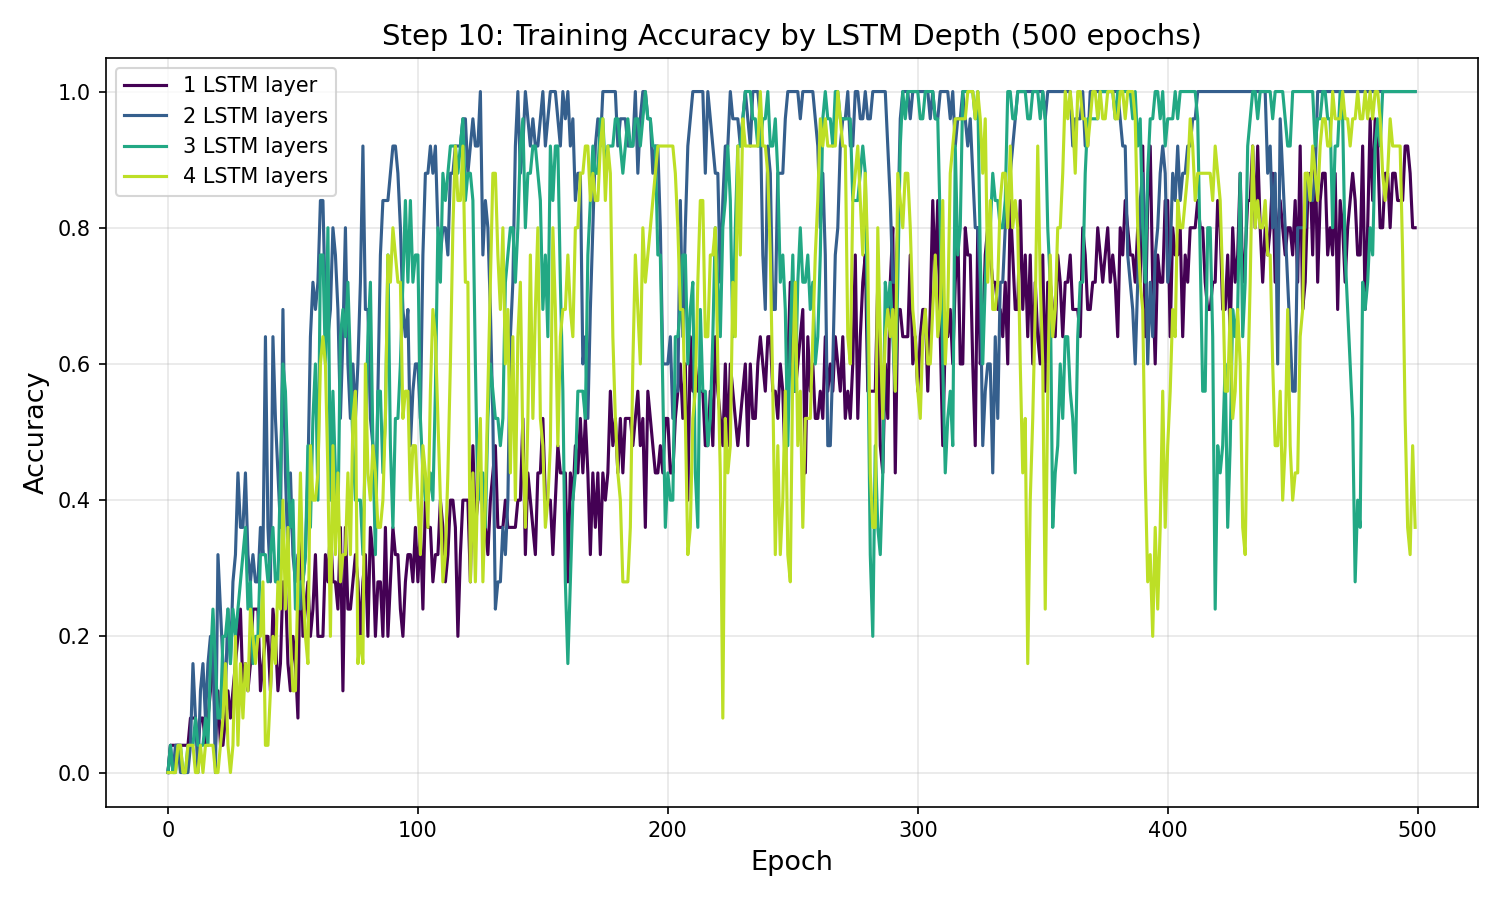
\includegraphics[width=0.90\textwidth]{step10_depth_accuracy.png}
  \caption{Training accuracy curves for 1--4 LSTM layers over 500 epochs. Depths 1--3
           converge to 100\%; depth 4 fails to converge within the epoch budget.}
  \label{fig:depth-acc}
\end{figure}

\begin{figure}[H]
  \centering
  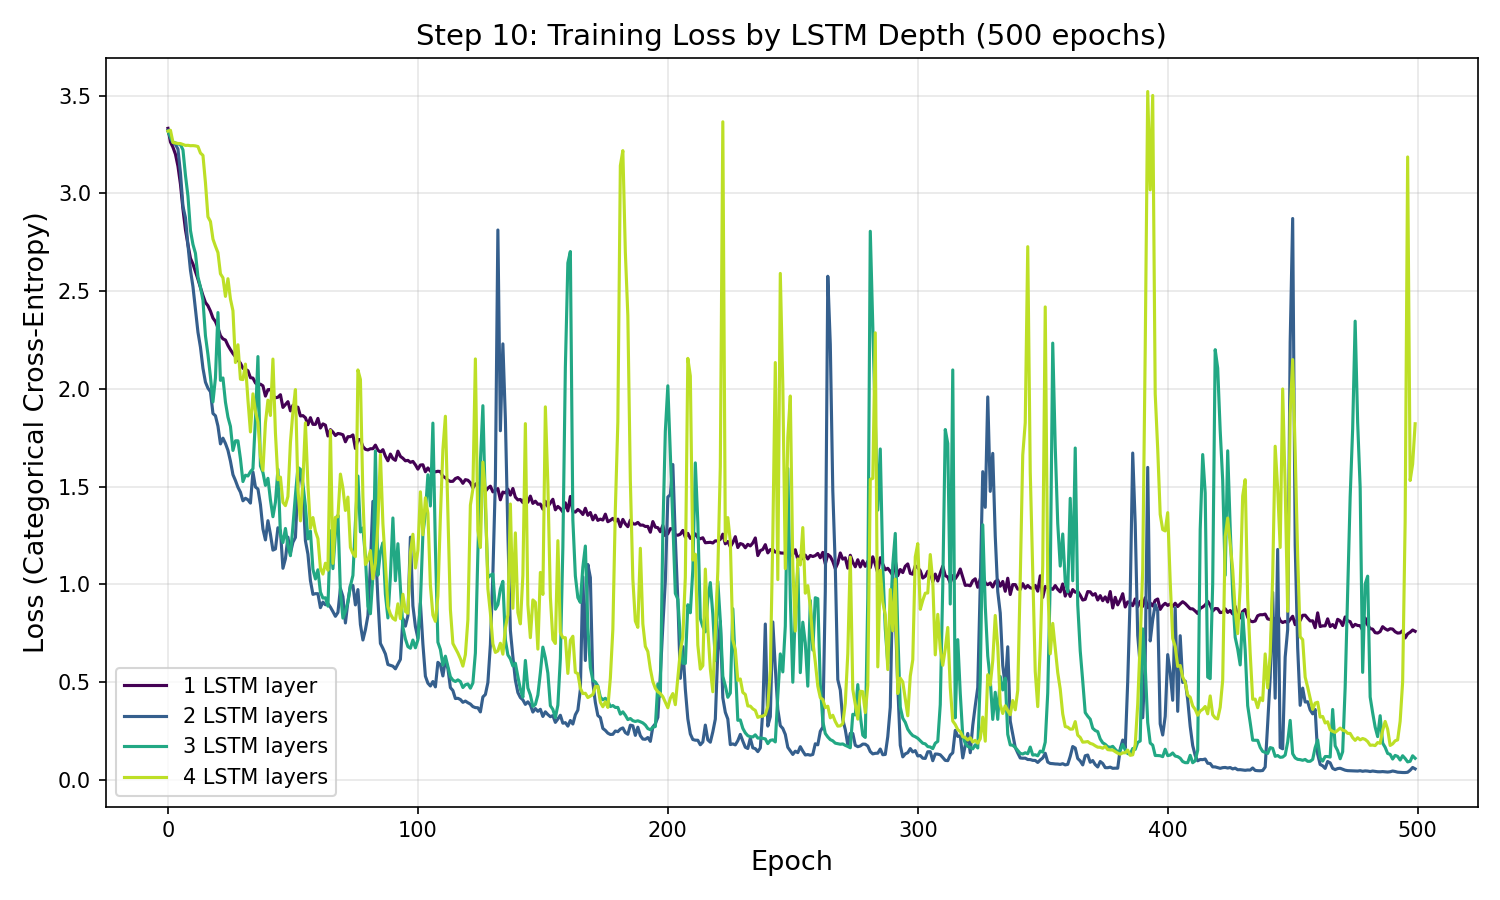
\includegraphics[width=0.90\textwidth]{step10_depth_loss.png}
  \caption{Training loss curves for 1--4 LSTM layers over 500 epochs. The 2-layer stacked
           LSTM achieves the lowest final loss.}
  \label{fig:depth-loss}
\end{figure}

\subsection{Hyperparameter Experiments (Step 11)}

Three independent sweeps were conducted, each varying one parameter while holding
others at the baseline (hidden=32, layers=1, lr=0.01, 500 epochs, batch=1).

\subsubsection{Sweep A: Learning Rate}

\begin{table}[H]
  \centering
  \caption{Effect of learning rate on final accuracy (hidden=32, layers=1, 500 epochs)}
  \label{tab:lr}
  \begin{tabular}{crr}
    \toprule
    \textbf{Learning Rate} & \textbf{Accuracy (\%)} & \textbf{Loss} \\
    \midrule
    0.0001 &   8.00 & 2.9093 \\
    0.001  &  84.00 & 1.6479 \\
    0.005  &  96.00 & 0.9989 \\
    \textbf{0.01}   & \textbf{100.00} & \textbf{0.6317} \\
    0.05   &  92.00 & 0.8086 \\
    0.1    &  96.00 & 0.5517 \\
    \bottomrule
  \end{tabular}
\end{table}

\textbf{Optimal: lr = 0.01.} Very small learning rates (0.0001) produce severe
underfitting within 500 epochs (8\% accuracy). The rate 0.001 reaches 84\% but leaves
headroom. Rates from 0.005--0.1 all exceed 80\%, but 0.01 uniquely reaches 100\%. Larger
rates (0.05, 0.1) converge faster initially but show slightly less complete memorisation
at epoch 500, suggesting mild oscillation near the optimum.

\begin{figure}[H]
  \centering
  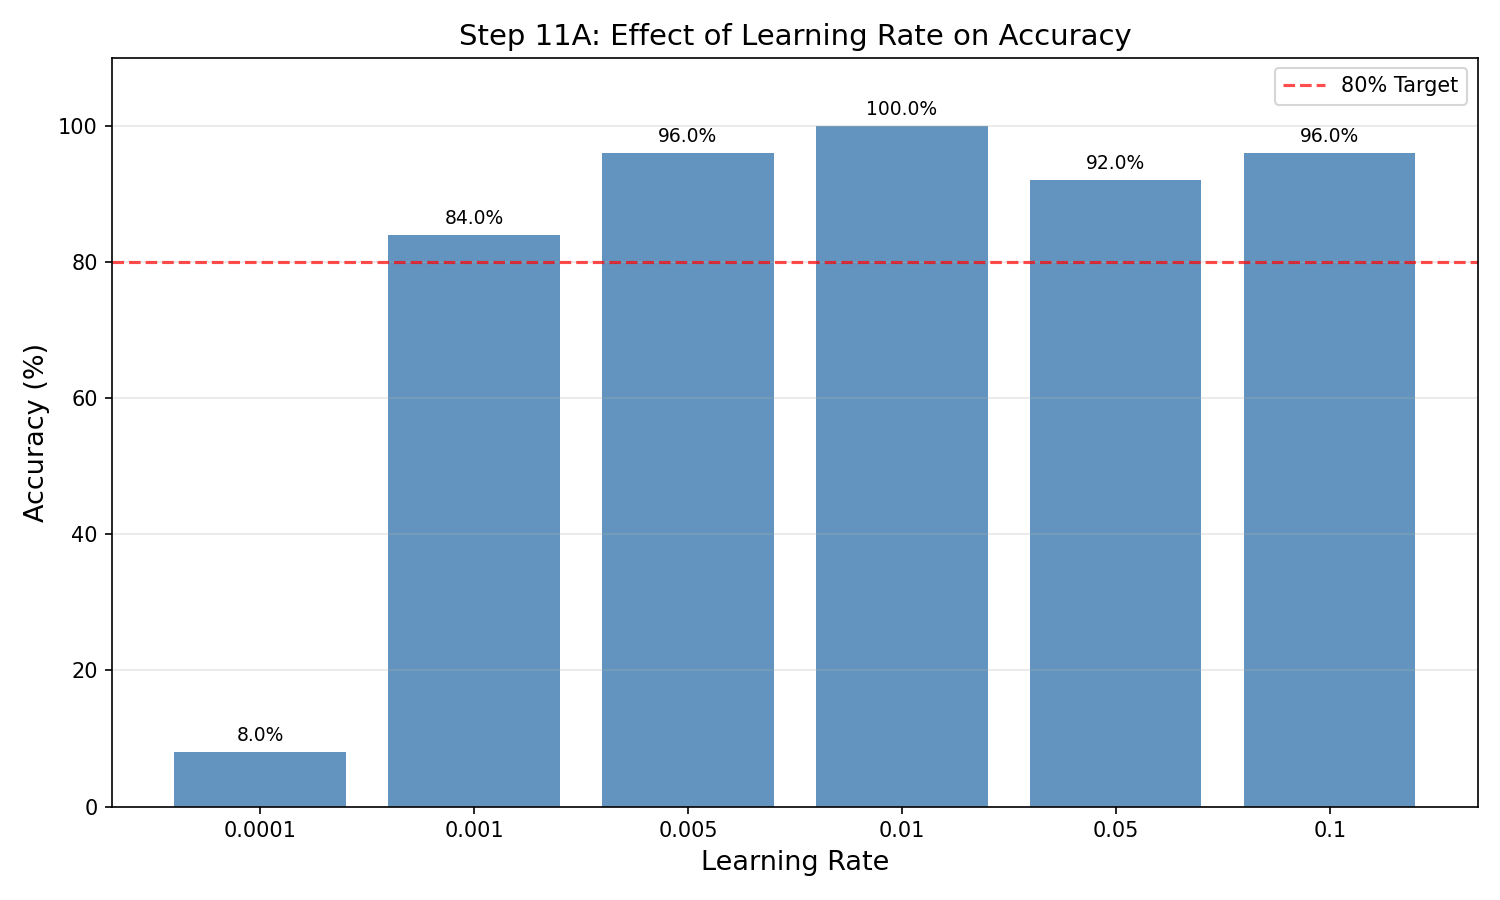
\includegraphics[width=0.90\textwidth]{step11_learning_rate.png}
  \caption{Effect of learning rate on final accuracy after 500 epochs. The red dashed
           line marks the 80\% target. lr=0.01 achieves 100\%.}
  \label{fig:lr}
\end{figure}

\subsubsection{Sweep B: Hidden Size}

\begin{table}[H]
  \centering
  \caption{Effect of hidden size on final accuracy (layers=1, lr=0.01, 500 epochs)}
  \label{tab:hidden}
  \begin{tabular}{crr}
    \toprule
    \textbf{Hidden Units} & \textbf{Accuracy (\%)} & \textbf{Loss} \\
    \midrule
    4   &  96.00 & 1.1923 \\
    8   &  96.00 & 0.8952 \\
    16  &  96.00 & 0.7905 \\
    \textbf{32}  & \textbf{100.00} & \textbf{0.6317} \\
    64  & 100.00 & 0.4624 \\
    128 & 100.00 & 0.3762 \\
    \bottomrule
  \end{tabular}
\end{table}

\textbf{Optimal: hidden = 32} (smallest size achieving 100\%; selected by parsimony).
Sizes 4--16 plateau at 96\% -- they lack sufficient representational capacity to
distinguish all 25 mappings. Sizes 32, 64, and 128 all achieve 100\%, with diminishing
loss improvement beyond 32. The baseline of 32 is chosen as the optimal value per the
Occam's razor principle: minimum necessary capacity.

\begin{figure}[H]
  \centering
  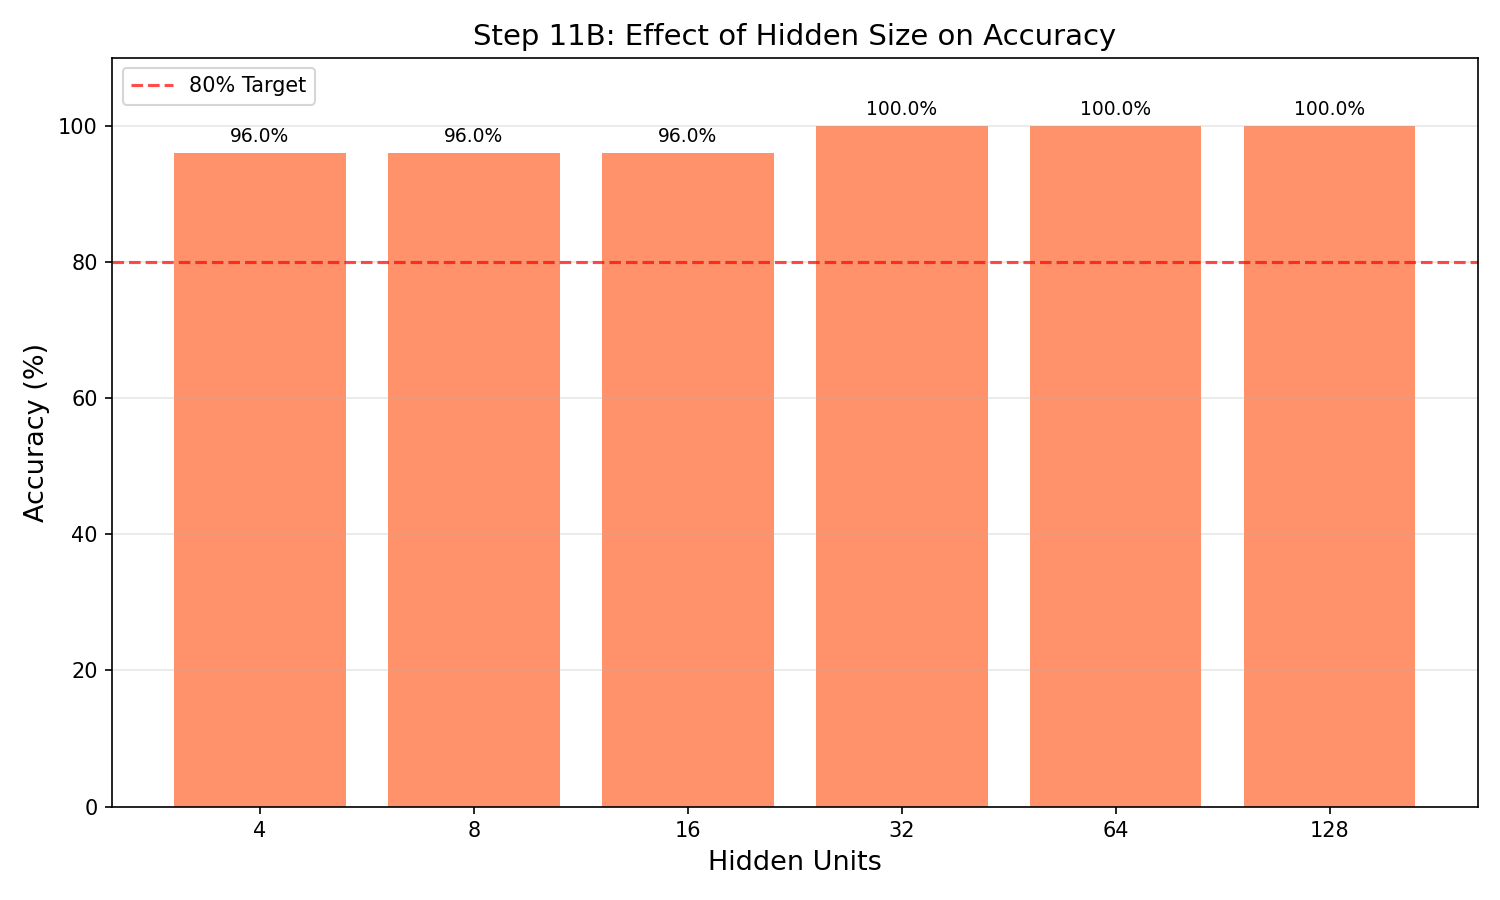
\includegraphics[width=0.90\textwidth]{step11_hidden_size.png}
  \caption{Effect of hidden layer size on final accuracy. Sizes $\geq32$ all achieve
           100\%; smaller sizes plateau at 96\%.}
  \label{fig:hidden}
\end{figure}

\subsubsection{Sweep C: Number of Layers (Hyperparameter Selection)}

\textit{Note: Step 10 examined convergence trajectories (epoch-by-epoch curves) for
architectural analysis. This sweep reports the single final-accuracy figure at epoch 500
for hyperparameter selection. The overlapping depth range serves a distinct analytical
purpose.}

\begin{table}[H]
  \centering
  \caption{Effect of number of layers on final accuracy (hidden=32, lr=0.01, 500 epochs)}
  \label{tab:layers}
  \begin{tabular}{crr}
    \toprule
    \textbf{Layers} & \textbf{Accuracy (\%)} & \textbf{Loss} \\
    \midrule
    \textbf{1} & \textbf{100.00} & \textbf{0.6317} \\
    2 & 100.00 & 0.0378 \\
    3 & 100.00 & 0.0822 \\
    4 &  40.00 & 1.8950 \\
    5 & 100.00 & 0.1530 \\
    \bottomrule
  \end{tabular}
\end{table}

\textbf{Optimal: layers = 1} (selected by parsimony). Layers 1, 2, 3, and 5 all achieve
100\% accuracy. Layer 4 fails to converge within 500 epochs, consistent with the Step 10
finding. Since the simplest model achieves perfect accuracy on this 25-sample task, adding
layers introduces unnecessary parameters and convergence risk without accuracy benefit.

\begin{figure}[H]
  \centering
  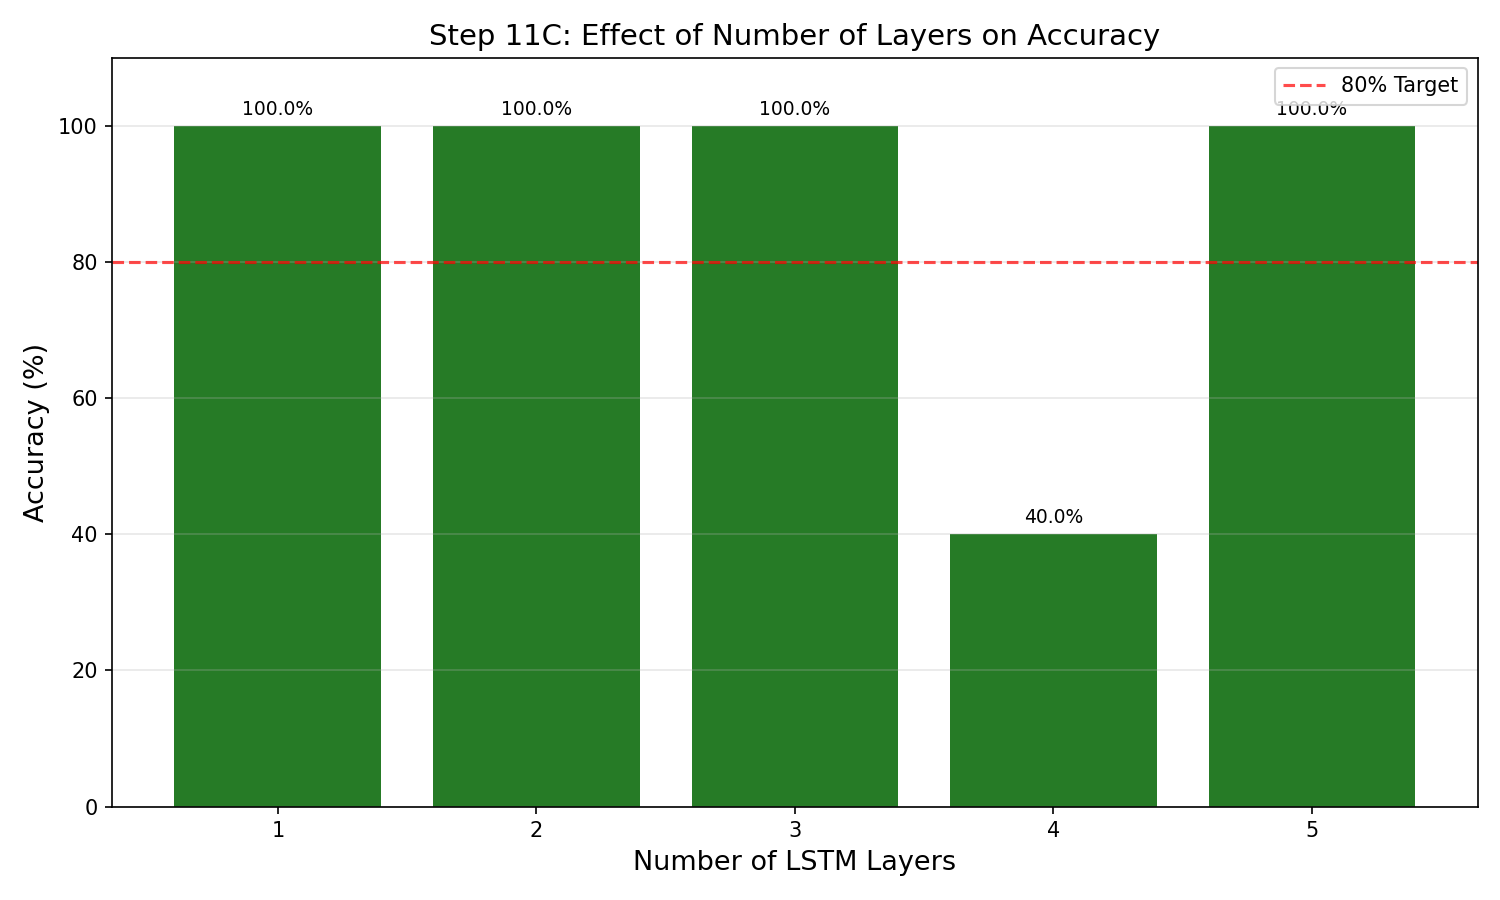
\includegraphics[width=0.90\textwidth]{step11_num_layers.png}
  \caption{Effect of number of LSTM layers on final accuracy. Most configurations
           achieve 100\%; depth 4 fails to converge within 500 epochs.}
  \label{fig:layers}
\end{figure}

% =============================================================================
\section{Analysis}
% =============================================================================

\subsection{Nature of the Task: Training-Set Memorisation}

This is a \textbf{training-set memorisation task}, not a generalisation benchmark. The
model is evaluated on the same 25 samples it was trained on, with no held-out test set.
Accuracy therefore reflects the model's ability to memorise 25 fixed input-output pairs,
not to generalise to unseen sequences. This is a deliberate design choice per the
assignment specification and is the standard framing for this pedagogical exercise.

\subsection{Single-Timestep Input and LSTM Recurrent Memory}

With \texttt{timesteps=1}, each of the 25 samples is processed in a single LSTM forward
pass. Because there is only one time step per sample, the recurrent connections carry no
information \emph{within} a sample: the hidden state computed at step $t=1$ is the final
hidden state, and there are no prior time steps to inform it. The task collapses into a
\textbf{one-step mapping problem} from a single normalised input scalar to one of 26
output classes. The LSTM's gating mechanism --- designed to selectively retain information
\emph{across multiple time steps} --- is not meaningfully exercised here.

The LSTM succeeds despite this limitation because:
\begin{enumerate}
  \item The 32-dimensional hidden projection provides sufficient capacity to encode 25
        distinct input-output mappings.
  \item Adam at lr=0.01 converges efficiently on this small problem.
  \item 500 epochs provide ample gradient updates for the 25-sample dataset.
\end{enumerate}

\subsection{Depth Trade-offs}

Adding LSTM layers increases both parameter count and gradient path length. On a
25-sample task, this introduces two risks:
\begin{itemize}
  \item \textbf{Over-parameterisation:} More weights than are needed to solve a trivial
        mapping task.
  \item \textbf{Slower convergence:} Gradients must flow through more LSTM gates, and
        the fixed 500-epoch budget may be insufficient. This is evident in the depth-4
        failure (40\% accuracy).
\end{itemize}
The step-10 convergence curves confirm that the 2-layer stacked LSTM converges faster
(lower loss at epoch 500) than the 1-layer baseline, while the 4-layer model diverges --
consistent with the over-parameterisation hypothesis.

\subsection{Hyperparameter Interactions}

\begin{itemize}
  \item \textbf{Learning rate} is the most impactful hyperparameter on this task. The
        range 0.005--0.1 all exceed 80\%, but only 0.01 achieves 100\% at epoch 500.
        The effect is strong: lr=0.0001 achieves only 8\%, confirming that the 500-epoch
        budget is the binding constraint at very small learning rates.
  \item \textbf{Hidden size} shows a capacity threshold. Below 32 units, the model lacks
        sufficient representational capacity for 25 distinct class mappings; at 32 and
        above, the task is within capacity and all sizes perform equally.
  \item \textbf{Depth} interacts with convergence budget: deeper models need more epochs
        or a higher learning rate to compensate for increased gradient path length.
\end{itemize}

% =============================================================================
\section{Conclusion}
% =============================================================================

The LSTM model successfully learns the alphabet sequence prediction task, achieving
\textbf{100\% accuracy} with the baseline configuration --- well above the 80\% target.
Key findings:

\begin{enumerate}
  \item The \textbf{baseline model} (1 LSTM layer, 32 hidden units, lr=0.01) correctly
        predicts all 25 next-letter mappings.
  \item The \textbf{2-layer stacked LSTM} (Step 10 spec anchor) also achieves 100\%
        accuracy with a lower final loss (0.0378 vs.\ 0.6317), indicating more complete
        convergence.
  \item \textbf{Depth 4 fails to converge} within 500 epochs, confirming that deeper
        networks require a larger training budget on this small dataset.
  \item \textbf{lr=0.01} is the optimal learning rate; lr=0.0001 produces severe
        underfitting (8\%) within the fixed epoch budget.
  \item \textbf{Hidden size 32} is the minimum capacity threshold for 100\% accuracy;
        smaller sizes plateau at 96\%.
  \item The \textbf{optimal configuration} is lr=0.01, hidden=32, layers=1 --- the
        simplest model that achieves perfect accuracy.
  \item This task is a \textbf{one-step mapping problem}: with a single input timestep,
        the LSTM's recurrent memory mechanism is not exercised. Accuracy reflects
        memorisation capacity, not sequential generalisation.
\end{enumerate}

% =============================================================================
\begin{thebibliography}{9}

\bibitem{hochreiter1997}
  Hochreiter, S. and Schmidhuber, J. (1997). \textit{Long Short-Term Memory.}
  Neural Computation, 9(8), pp.\ 1735--1780.

\bibitem{chollet2018}
  Chollet, F. (2018). \textit{Deep Learning with Python.} Manning Publications.

\bibitem{keras}
  Keras documentation --- LSTM layer.
  \url{https://keras.io/api/layers/recurrent_layers/lstm/}

\end{thebibliography}

\vspace{1em}
\noindent\small\textit{%
Code: \texttt{Assignment 3/code/assignment3.py}\quad
Plots: \texttt{Assignment 3/output/}\quad
Result tables: \texttt{output/baseline\_results.txt}, \texttt{step10\_depth\_results.csv},
\texttt{step11\_*.csv}%
}

\end{document}
